\documentclass[12pt, a4paper]{article}
\usepackage[utf8]{inputenc} % uft8 you know
\usepackage[danish]{babel}
\usepackage{lastpage}
\usepackage{fancyhdr}
\usepackage{hyperref}
%\usepackage{biblatex}
\usepackage[T1]{fontenc}
\usepackage{ae}
\usepackage{graphicx}
\usepackage{pdfpages} % Til at inkludere pdf'er
\usepackage{amsmath}
\usepackage{amsfonts}
\usepackage{amssymb}
\usepackage{longtable}
\usepackage{adjustbox}
\usepackage{blindtext}
\usepackage[margin=2.7cm]{geometry}
\usepackage{tabularx, booktabs, siunitx}
\usepackage{multirow}
\usepackage{natbib} % Works with.bib files
\usepackage{listings}
\usepackage{xcolor}
\usepackage{placeins}
\usepackage{listings}

\bibliographystyle{apalike} 
% Define custom settings for C++ code
\lstset{
	language=C++, % Set the language to C++
	basicstyle=\ttfamily\small, % Use a monospaced font
	numbers=left, % Line numbers on the left
	numberstyle=\tiny\color{gray}, % Line number style
	stepnumber=1, % Line number increment
	numbersep=5pt, % Space between line numbers and code
	backgroundcolor=\color{lightgray!10}, % Light gray background
	showspaces=false, % Don't show spaces
	showstringspaces=false, % Don't mark spaces in strings
	showtabs=false, % Don't show tab characters
	frame=single, % Single-line frame around code
	rulecolor=\color{black}, % Frame color
	tabsize=2, % Tab size
	captionpos=b, % Caption position (bottom)
	breaklines=true, % Allow breaking lines
	breakatwhitespace=false, % Only break at whitespace if true
	keywordstyle=\color{blue}, % Keywords in blue
	commentstyle=\color{green!60!black}, % Comments in green
	stringstyle=\color{red}, % Strings in red
}

%\geometry{
%	total={170mm,257mm},
%	left=20mm,
%	top=30mm,
%	bottom=30mm,
%}
\hypersetup{
    pdftitle={Sådan bygger du din egen datalogger - Science klubben},
    pdfauthor={Science klubben - Kristoffer Sørensen, Felix Jensen},
    % Remove the red border around links
    pdfborder={0 0 0},
}

\pagestyle{fancy} % definds the pagestyleing
\renewcommand{\headrulewidth}{0pt} % Removes the line under the header

\fancyhead{}
\fancyhead[l]{Science Klub - Datalogger}
\fancyhead[r]{\today}
\fancyfoot{}
\fancyfoot[C]{Side \thepage\ af \pageref{LastPage}}
%\fancyhf{} % Removes the wired header text
%\cfoot{Side \thepage\ af \pageref{LastPage}} % Sets the right side of the footer to "Page X of Y"
%\lhead{Gruppe 1} % Sets the left side of the header to "Gruppe 1"

\begin{document}
    %\providecommand\NAT
    \title{
    Arbejdsgruppe i Science klubben\\ 
    Sådan byggede vi vores egen datalogger\\
}

\author{Af Science klubbens medlemmer}
\maketitle

\begin{figure}[!h]
	\centering
	\includegraphics[width=0.45\textwidth]{Figures/TMP.MP}
	\caption{Arduinoen i virkeligheden under udvikling}
\end{figure}

\thispagestyle{empty}
    \newpage
    \tableofcontents
    \newpage
    
    \section{Introduktion}\label{sec:introduktion}
	Dette projekt er støttet af NNF (Novo Nordisk Fonden) og formålet med det generelle projekt er at lade elever prøve at arbejde som forskere. Dertil har eleverne udviklet en station som skulle indsamle data. Dataet bliver behandlet af lærere på Rybners HTX, som vil blive brugt i undervisningsforløb til folkeskoler og arbejdsopgaver til gymnasiet. Denne arbejdsgruppe arbejder med at opbygge en datalogger, som skal kunne indsamle diverse data via forskellige sensorer. Dette dokument beskriver, hvordan hver sensor er sat op, hvilke kodevalg der er blevet gjort, og hvordan programmet bliver kørt igennem. Hvert kapitel i dokumentet, efter Kode og Flowcharts, angiver en sensor og hvordan den er sat op. 
	\subsection{Forbindelser i Arduinoen}
		Her er et overblik over hvilke porte som er i brug på Arduino Mega'en. Der er blevet brugt et program kaldet Fritzing til at visualisere, hvordan de forskellige sensorer og moduler er forbundet til Arduinoen (Se kapitel \ref{sec:VisuelDatalogger}). På grund af det høje antal af moduler og kabler er der oplyst herunder for hvert modul, hvor og hvordan det enkelte modul er forbundet til Arduinoen. (Det vil også stå inde under hver moduls sektion)\\ [7pt]
		\begin{minipage}{0.49\textwidth}
			RTC (Real Time Clock):
			\begin{itemize}
				\item 5V - 5V
				\item GND - GND
				\item SCL - Port 21 (SCL)
				\item SDA - Port 20 (SDA)
			\end{itemize}
			SD Card Module:
			\begin{itemize}
				\item +5 - 5V
				\item +3.3 - 3.3V
				\item GND - GND
				\item CS - Port 53 (SS)
				\item MOSI - Port 51 (MOSI)
				\item SCK - Port 52 (SCK)
				\item MISO - Port 50 (MISO)
			\end{itemize}
		\end{minipage}
		\hfill
		\begin{minipage}{0.49\textwidth}
			Digital Temperatur Sensor (DS18B20):
			\begin{itemize}
				\item Rød ledning - 5V
				\item Sort ledning - GND
				\item Gul ledning - 5V $\to$ 1K$\Omega$ resistor $\to$ Port 22
			\end{itemize}
			pH Sensor:
			\begin{itemize}
				\item V+ - 5V
				\item G - GND
				\item PO - A0
				\item TO - A1
			\end{itemize}
		\end{minipage}
		\newpage
		\begin{minipage}{0.49\textwidth}
			UV Sensor (VEML6075):
			\begin{itemize}
				\item 3Vo - 3.3V
				\item GND - GND
				\item SCL - Port 21 (SCL)
				\item SDA - Port 20 (SDA)
			\end{itemize}
			Tryksensor (MLP3115A2):
			\begin{itemize}
				\item 3Vo - 3.3V
				\item GND - GND
				\item SCL - Port 21 (SCL)
				\item SDA - Port 20 (SDA)
			\end{itemize}
		\end{minipage}
		\hfill
		\begin{minipage}{0.49\textwidth}
			MQ2 Gas Sensor:
			\begin{itemize}
				\item VCC - 5V
				\item GND - GND
				\item NC - N/A
				\item SIG(AO) - A2
			\end{itemize}
		\end{minipage}
		
	\newpage
	\subsubsection{Opbygning af datalogger visualiseret}\label{sec:VisuelDatalogger}
		\begin{figure}[h!]
			\centering
			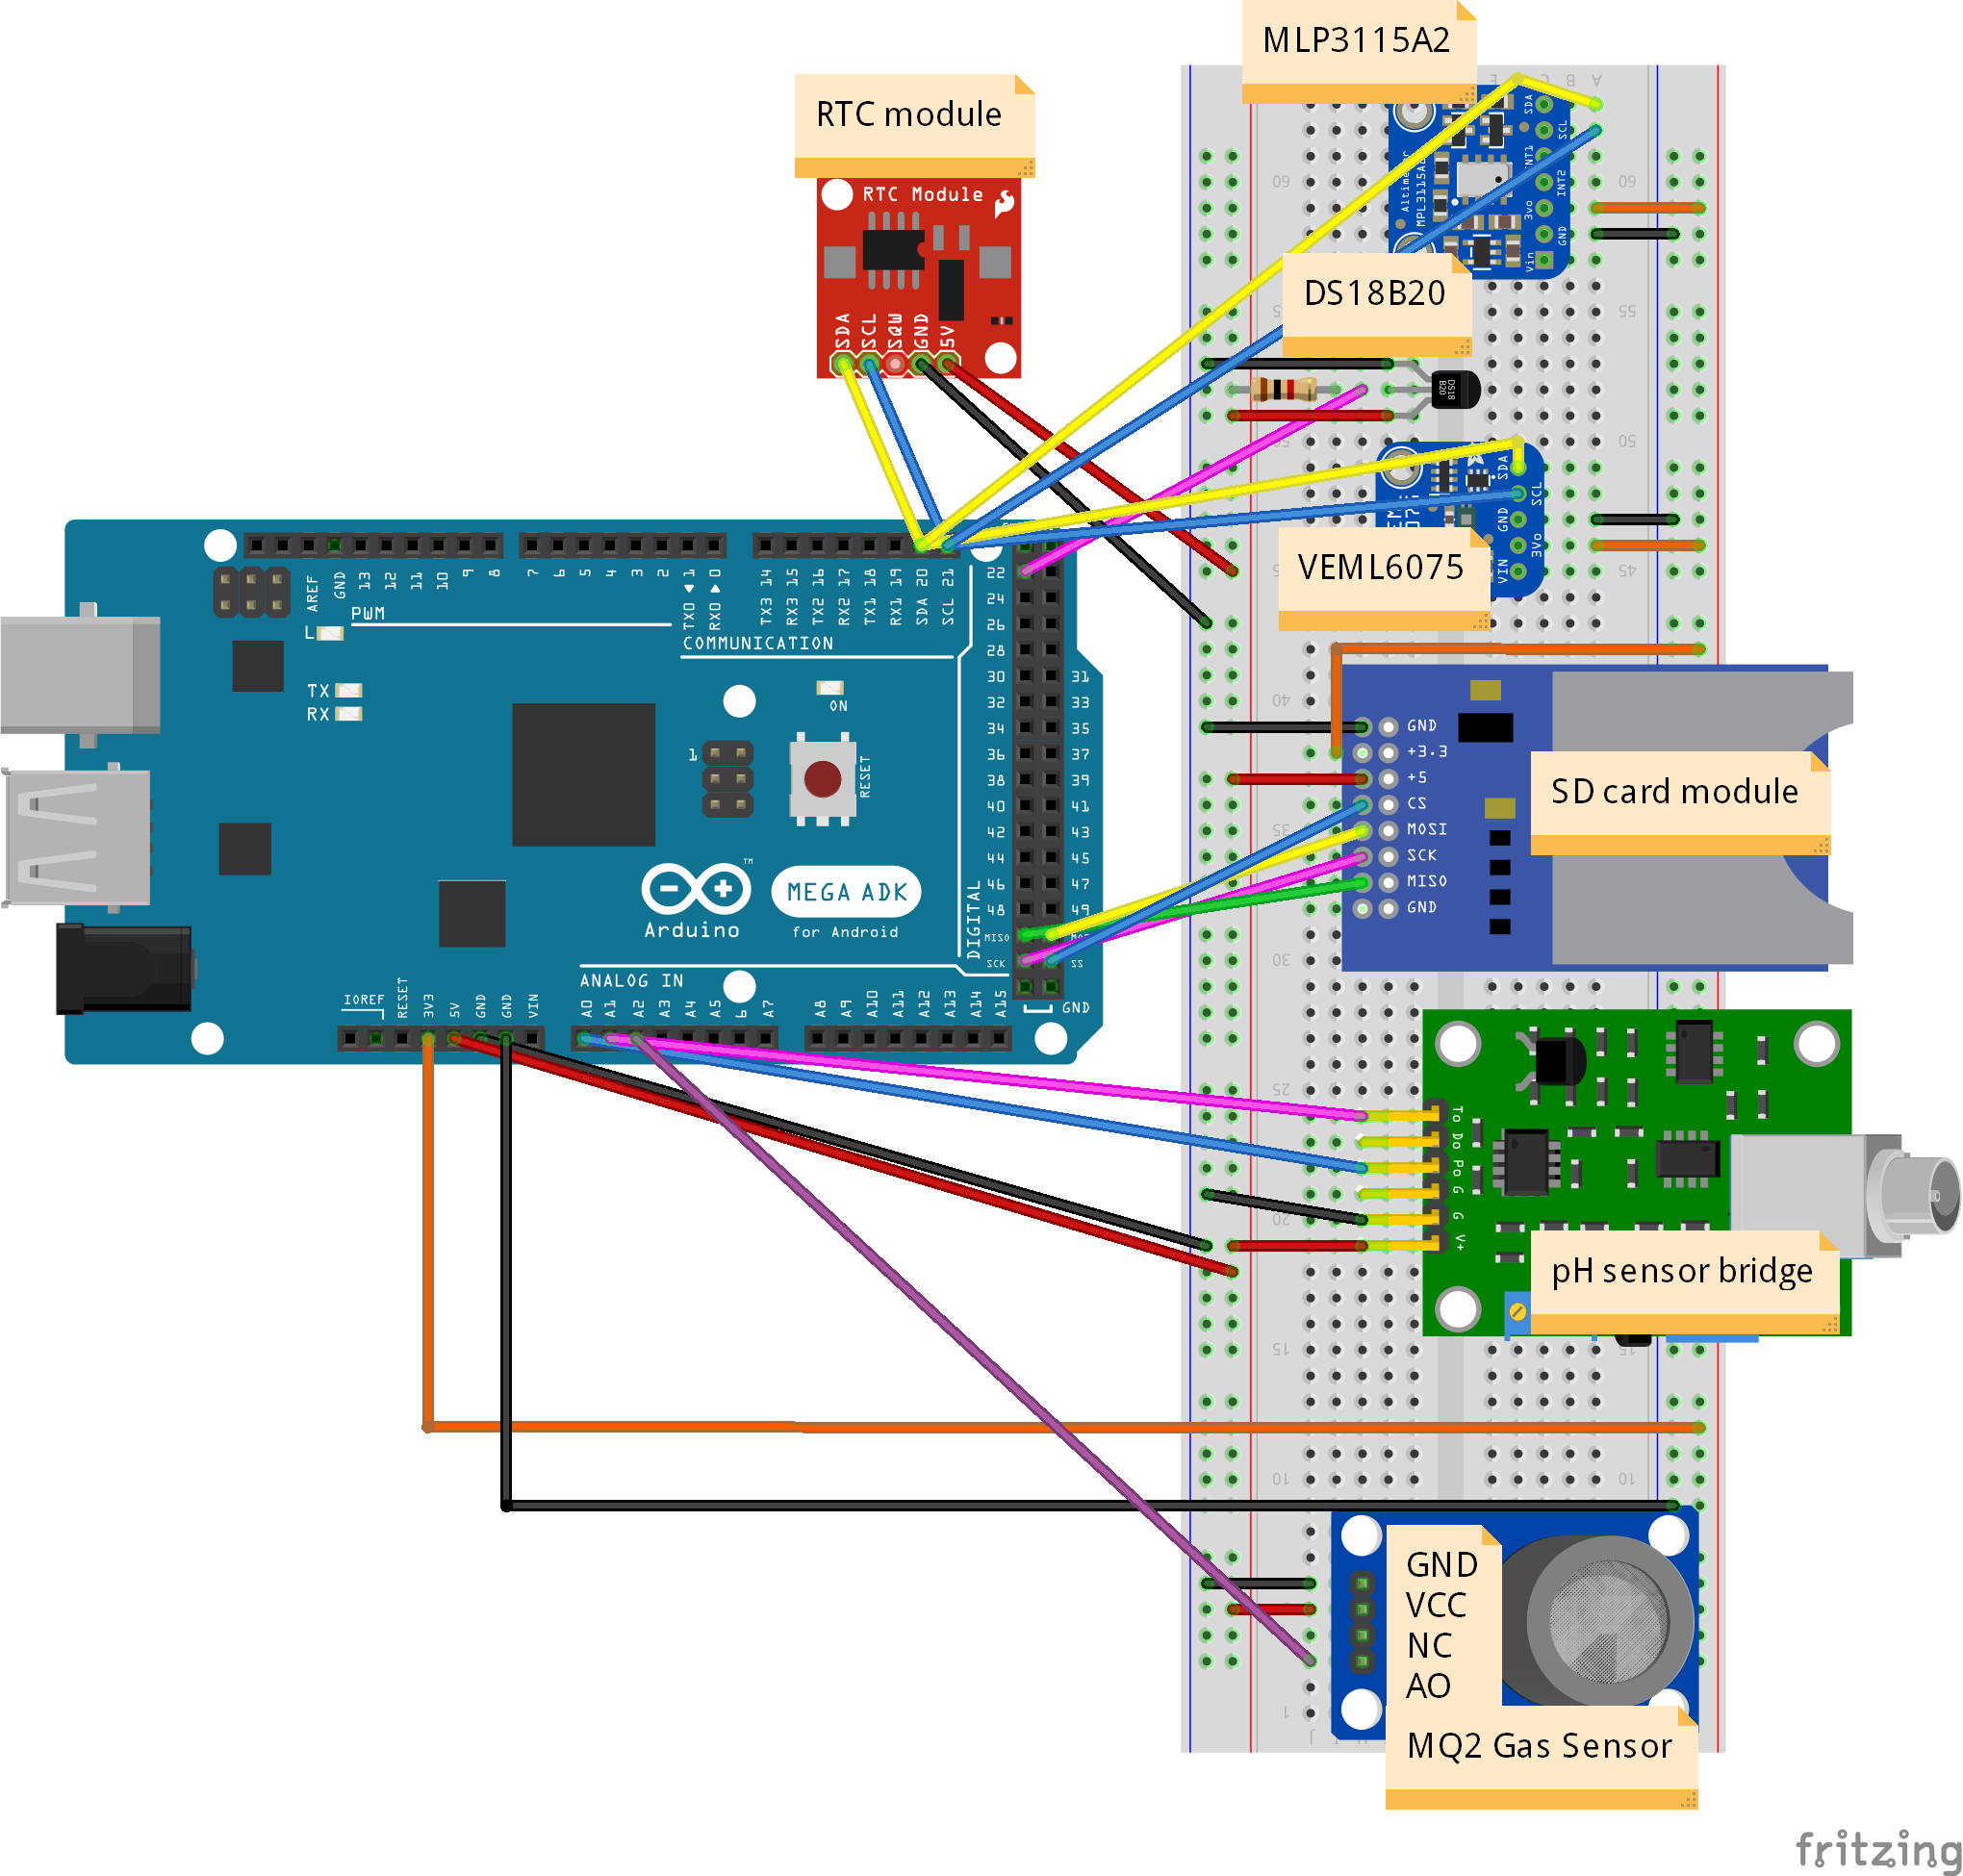
\includegraphics[width=\textwidth]{Figures/Diagram_v3.png}
			\caption{Opstillingen af nuværende datalogger lavet i Fritzing m. Arduino og moduler} \label{fig:Opstilling}
		\end{figure}
    
    \newpage
    \clearpage
    \section{Kode og Flowcharts}
	\subsection{Flowcharts}
		\begin{figure}[!h]
			\centering
			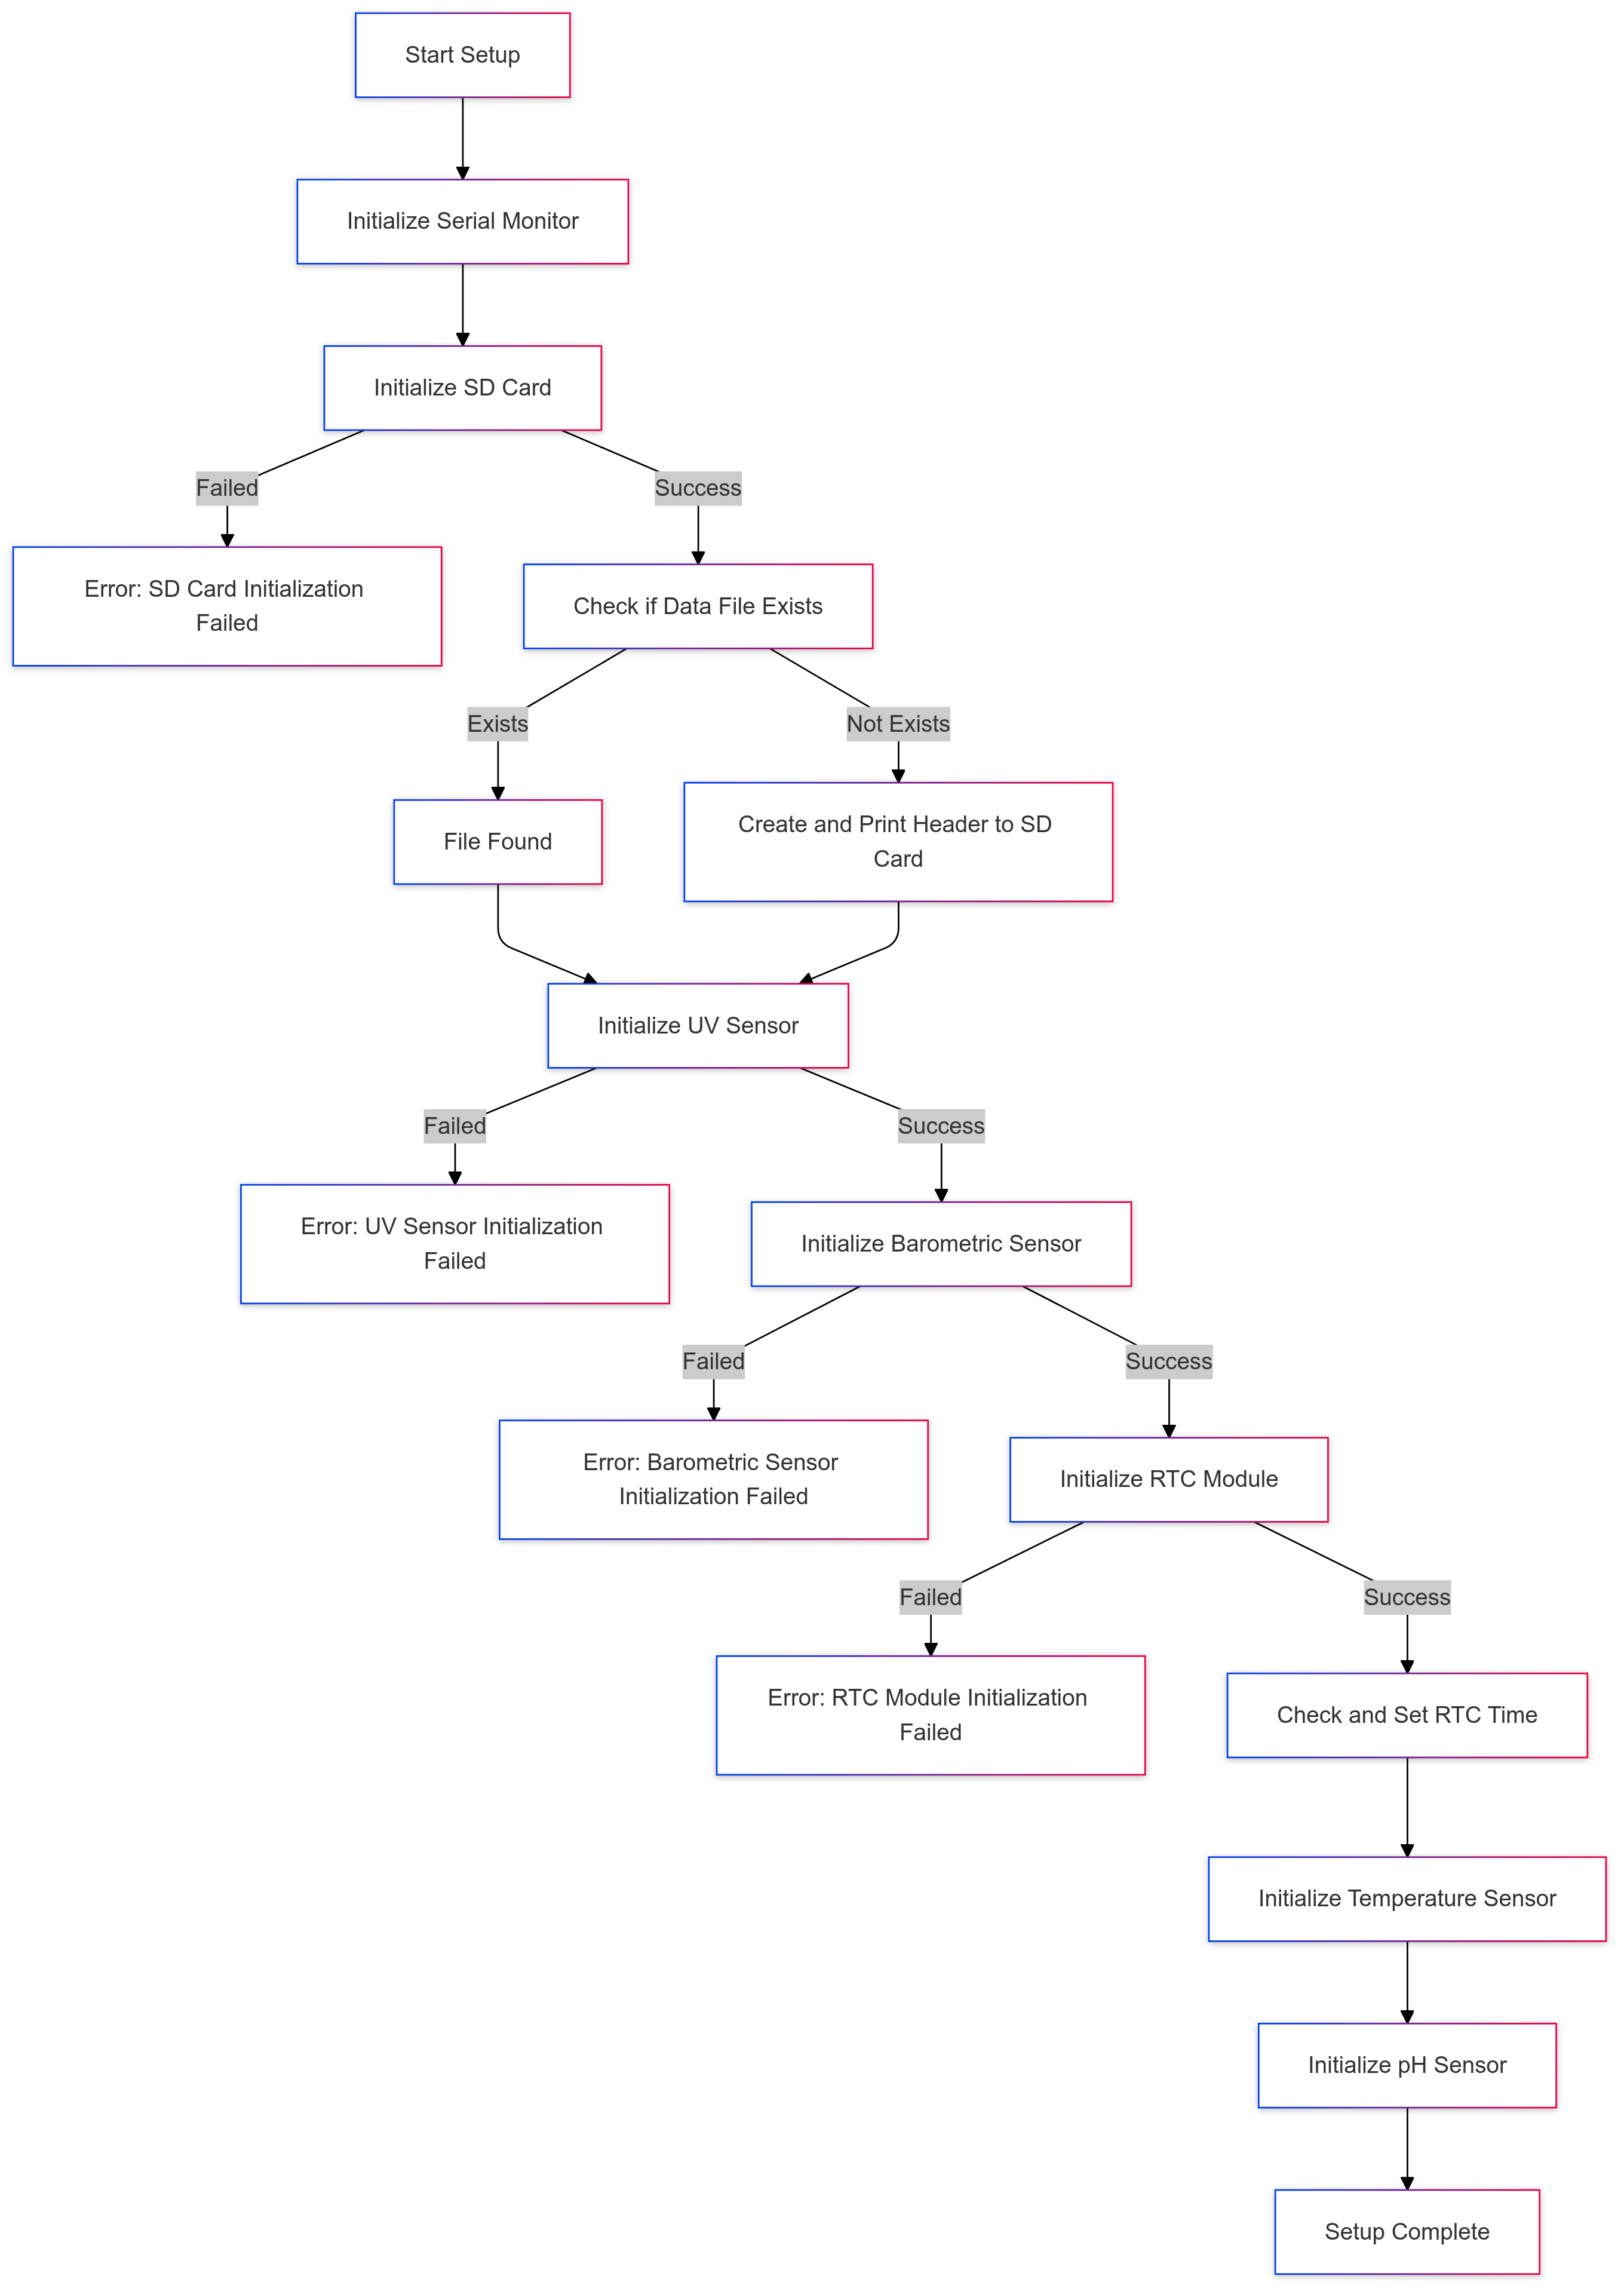
\includegraphics[width=0.9\textwidth]{Figures/Flowchart setup.png}
			\caption{Flowchart til setup funktionen}
		\end{figure}
		
		\begin{figure}[!h]
			\centering
			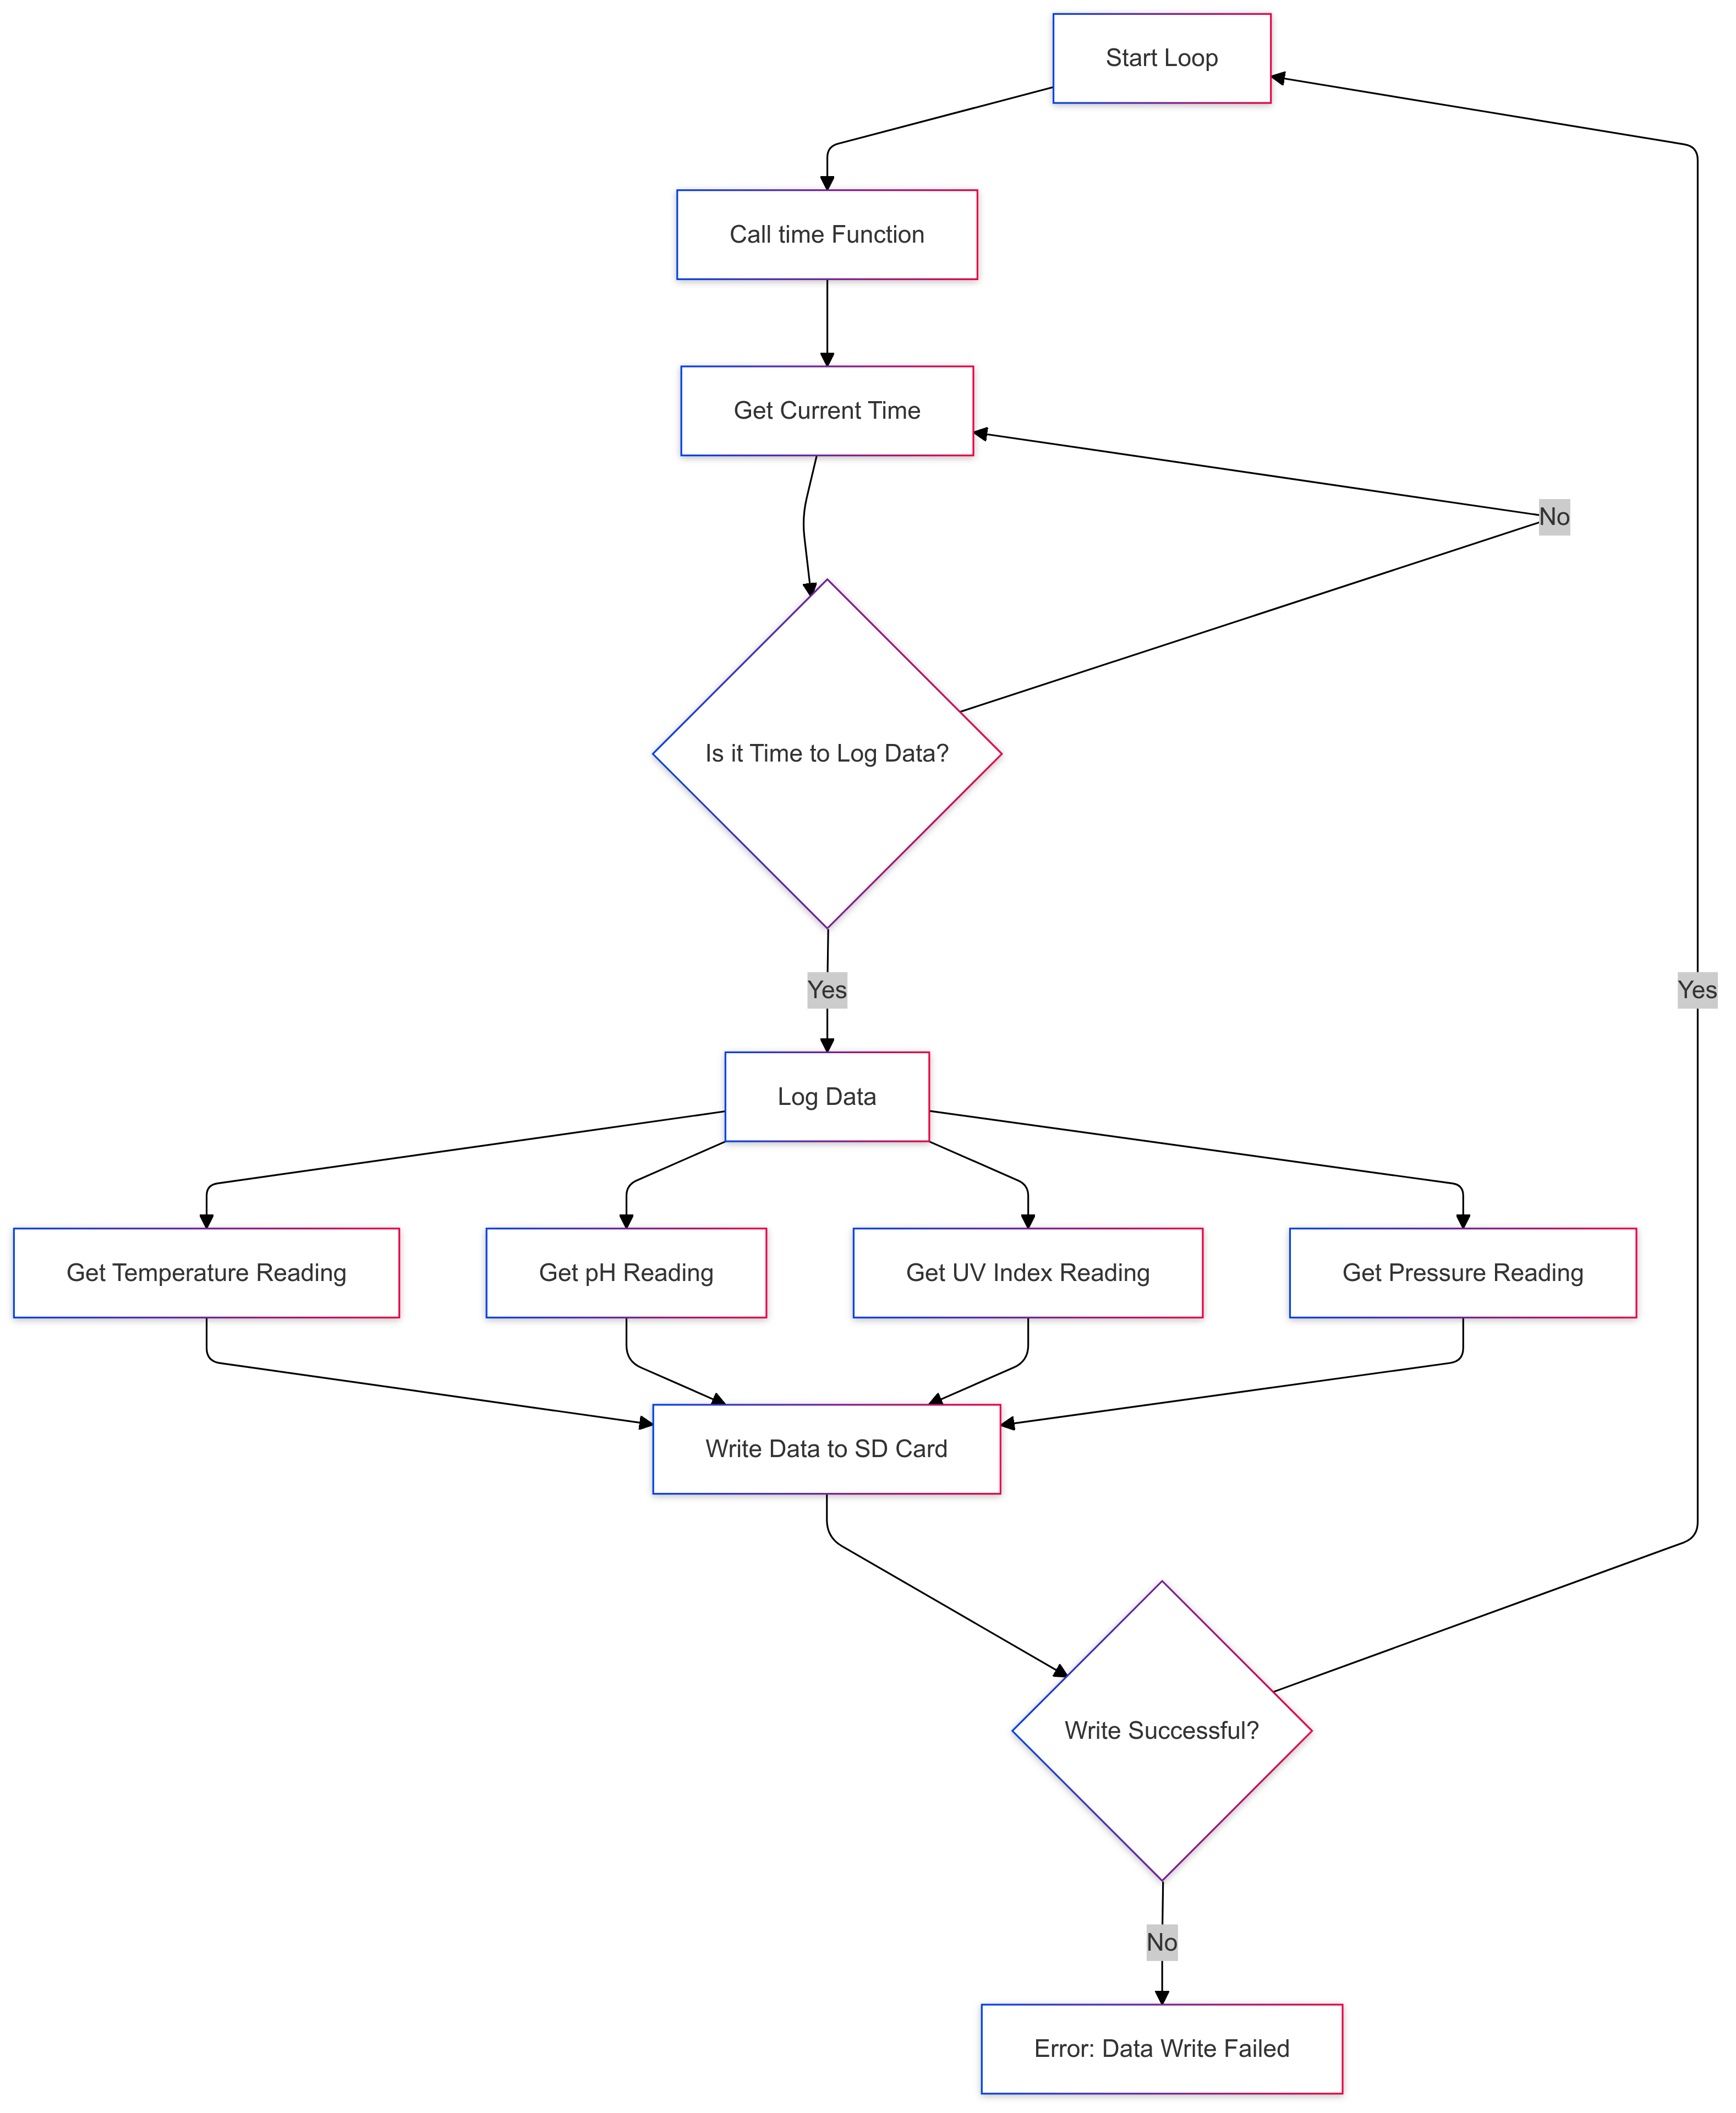
\includegraphics[width=\textwidth]{Figures/Flowchart loop.png}
			\caption{Flowchart til loop funktionen}
		\end{figure}
		
	\clearpage
	\newpage
	\subsection{Kode beskrivelse}
		Til koden er der importeret 9 biblioteker, hvor 7 af dem er til direkte brug af alle modulerne forbundet til Arduinoen.\\ [7pt]
		% Test koden uden de 2 sidste biblioteker
		Lige før setup funktionen bliver der defineret nogle globale variabler. Disse variabler er numrene på de pins, hvor modulerne er forbundet, navn på data filen som skal skrives til, tidsintervallet mellem måling af data, og nogle instanser, som giver nogle funktioner man kan bruge til at kommunikere med modulerne og sensorerne. En instans giver den defineret variabel nogle funktioner, som kan bruges. Det er funktioner, som bliver brugt ofte, og derfor er det lavet til noget, som kan kopires let. Eksempelvis er der i biblioteket, der hedder "Adafruit\_VEML6075.h"{} defineret en klasse, som hedder "Adafruit\_VEML6075"{}. Denne klasse har nogle funktioner i sig, og når man laver en instans af dette, hvilket f.eks. er gjort med variablen "uv"{}, så kan man tilgå alle klassens funktioner via variablen.
		\begin{lstlisting}
Adafruit_VEML6075 uv = Adafruit_VEML6075();
		\end{lstlisting}
		\vspace{15pt}
		Setup funktionen er en funktion, som kun bliver kørt én gang, når man starter Arduinoen eller genstarter koden. I setup funktionen sendes beskeder til alle modulerne som bruges, så de starter op og kan bruges. Et eksempel er, hvor der bliver kaldt "uv.begin()". Som forklaret ovenover, er uv en instans af en klasse med mange funktioner i, og .begin() er en af funktionerne, som kan bruges.\\ [5pt]
		I setup bliver der tjekket om der allerede findes en fil ved det navn, der er defineret. Man kan vælge at slette filen, hvis man gerne vil det. Det er der dog ikke behov for ved denne datalogger. Der bliver tjekket, om der findes en fil ved det defineret navn, fordi der skal tilføje en header linje til data filen, hvis det er tilfældet. Hvis Arduinoen startes op, og der allerede findes en fil ved det defineret navn, betyder det, at der allerede er data i filen. Derfor tilføjes der ikke en header linje. Hvis der ikke allerede er en fil ved det defineret navn, oprettes der en fil, og tilføjes en header linje, hvilket er navnene på dataet i hver kolonne, for at forklare, hvad de forskellige kolonners data er.
		\begin{lstlisting}
void header() {
	int attempts = 0;
	while (!writeToSDCard("Date, Time, Temperature, pH Value, UV Index, Pressure (hPa)\n")) {
		attempts++;
		// If the function could not print to the SD card after 10 tries, then it gives up
		if (attempts > 10) {
			Serial.println("Could not print the header to the SD card");
			return;  // Exits the function
		}
		delay(500);  // Adds a delay of 0.5 sec before retrying
	}
	Serial.println("Header printed successfully");
}
		\end{lstlisting}

		\newpage
		Loop funktionen er en funktion, som Arduinoen kører igen og igen. Fra denne funktion bliver man sendt videre til en anden funktion, som hedder "time". I time funktionen bliver RTC modulet kaldt, for at få tiden givet. Efter dette kører et loop for at vente x minutter, så der er en pause mellem målingerne fra modulerne. Det var muligt at bruge den indbygget delay() funktion til at vente en mængde tid, men det ville ikke være muligt at køre noget andet på Arduinoen imens. Efter tiden er gået, bliver logdata funktionen kaldt, og to tekst værdier bliver givet til funktionen. Det er dato og tid, så det kan skrives ind i filen på SD kortet sammen med dataet. \\ [7pt]
		Til hver af sensor modulerne er der lavet en funktion, som giver værdien for hver af sensorerne (For at se koden, gå ned til modulets beskrivelse nedenunder og se kode eksemplet). Disse værdier bliver sendt videre til writeToSDCard funktionen. Alle værdier fra sensorerne samt dato og tid bliver sat sammen til én stor tekst værdi (String) og sendt videre til writeToSDCard funktionen.
		\begin{lstlisting}
writeToSDCard(date + " " + time + "," + temperature + "," + pHValue + "," + uvValue + "," + pressureValue + "\n");
		\end{lstlisting}
		writeToSDCard tager én tekst værdi. Denne tekst værdi bliver sat direkte ind i filen på SD kortet vha. writeToSDCard funktionen. Den starter med at "åbne"{} SD kortet med ".open()"{} funktionen, og den forbindelse bliver gemt i en variabel, som gør det muligt at skrive til filen. For flere detaljer om at skrive til et SD kort, se sektion \ref{sec:SDCode}. Funktionen giver en sandt/falsk værdi tilbage (Boolean værdi), for at gøre det muligt at tjekke om der er skrevet til SD kortet. Den værdi bliver kun brugt i header funktionen, for at prøve at skrive kolonneoverskrifterne igen, hvis den fejler. Når writeToSDCard funktionen er færdig, så går koden bagud og gør logdata funktionen færdig, og time funktionen færdig. Arduinoen er nu tilbage i loop funktionen, som nu også er færdig, hvilket betyder, at den kalder loop funktionen igen. (For at se koden, se filen "Datalogger.ino")
		
	\subsection{Kode valg}
		Koden er opdelt i mange funktioner, fordi det gør det lettere at holde styr på hvad de enkelte dele gør. Når der er fejl er det også lidt lettere at finde delene med fejl. Der er lavet mange fejlhåndteringer for at koden kan skrive, hvilke fejl der opstår, og hvor. Der bliver brugt mange biblioteker skrevet af andre. Fordelene med dette er, at man ikke behøver at skrive meget kode selv. Ulemperne er dog, at man ikke kan være sikker på, at det virker. \\ [7pt]
		Dataet bliver skrevet til en .csv fil på SD kortet. Det er, fordi en .csv fil kan åbnes i et Excel ark. Hvis man vælger at skrive et program til at behandle dataet, er .csv meget let at arbejde med.\\ [15pt]
		\underline{Husk at ændre "delayInMinutes"{} variablen til det antal minutter I vil have mellem hver måling.}\\ [7pt]
		Download koden fra GitHub: \textit{\url{https://github.com/Felix-J07/Datalogger}}\\
		Eller se koden i sektion \ref{sec:Koden}
    \newpage
    \clearpage
    \section{RTC Module (Real Time Clock)}
	RTC er et modul, som kan holde styr på tiden meget præcist. Modulet bruges til at få en tid og en dato til hver måling af sensorerne. \\ [7pt]
	Sensoren har 4 pins der skal forbindes med Arduinoen. 5V, Ground, SDA og SCL. På Arduino Mega er port 20 ment som en SDA port og port 21 er ment som en SCL port. Hvis der er flere sensorer, som har SDA og SCL pins, så kan de alle sammen samles og tilkobles til port 20 og 21.
	\subsection{Kode}
		For at RTC modulet kan virke, er der brug for biblioteket, der hedder "RTClib.h". Herefter defineres i koden, før setup funktionen, hvilke porte SCL og SDA pins er tilkoblet til og der laves en instans af typen "RTC\_DS1307". Herefter initialiseres RTC modulet med en af instansens funktioner, "begin()". Herefter bliver der lavet tests for at se, om modulet virker. For at få tiden og datoen, kalder man en anden af objektets funktioner, "now()". Den funktion giver en "DateTime"{} værdi tilbage, som man kan gå ind i og få mere specifikke tidsoplysninger, såsom årstal, minuttal eller sekunder.
		
		\begin{lstlisting}
#include <RTClib.h>
#include <Wire.h>
#include <SPI.h>

RTC_DS1307 rtc;

// RTC config
const int rtcSDA = 20;
const int rtcSCL = 21;

void setup() {
	// Console config
	Serial.begin(9600);
	
	// Initializes the rtc module
	if (!rtc.begin()) {
		Serial.println("Couldn't find RTC");
		while (1)
		;
	}
	
	// Checks the time from the module
	DateTime now = rtc.now();
	if (now.year() < 2000) {
		Serial.println("RTC lost power, let's set the time!");
		// Following line sets the RTC to the date & time this sketch was compiled
		rtc.adjust(DateTime(F(__DATE__), F(__TIME__)));  // This is the line that sets the time to the time the code was compiled, if you want to change it you can do it here!
	}
}

void loop() {
	DateTime time = rtc.now();
	// Print YYYY-MM-DD
	Serial.println(String(time.year()) + "-" + time.month() + "-" + time.day());
	// Print HH-MM-SS
	Serial.println(String(time.hour()) + "-" + time.month() + "-" + time.second());
	delay(1000);
}
		\end{lstlisting}
    \newpage
    \clearpage
    \section{SD Card Module}
	SD modulet er det vigtigste modul i hele dataloggeren. Den gør det muligt at skabe en forbindelse mellem Arduinoen og SD-kortet. Dette betyder også, at hvis modulet ikke virker, så vil selve dataloggeren ikke virke. Når den måler data, skal den have et eksternt lager, for at lagre dataet. \\ [7pt]
	Sensoren har 7 pins, der skal forbindes med Arduinoen. 5V, 3.3V (optional), Ground, CS, MOSI, SCK, MISO. På Arduino Mega er porte 50 -- 52 reserveret til netop disse funktioner. SCK til 52, MOSI til 51, MISO til 50. CS kan forbindes til hvilken som helst pin på Arduinoen, men koden nedenunder er skrevet således, at CS skal være forbundet til port 53.\\ [7pt]
	Dette modul har skabt mange problemer undervejs i udviklingen. Dette er en tjekliste for at teste modulet, hvis den ikke virker:
	\begin{itemize}
		\item Sørg for at der er nok strøm til Arduinoen, så der vil være nok strøm til modulet
		\item Sørg for, at ledningerne sidder ordenligt
		\item Sørg for, at SD kortet fungerer, er formateret korrekt og er sat rigtigt i modulet
	\end{itemize}
	Hvis modulet stopper med at fungere efter der er påsat flere sensorer, prøv at flytte SD Kort Modulet over til en tom Arduino. Hvis den ikke virker på den tomme Arduino, betyder det højest sandsynligt, at modulet ikke virker.
	 
	\subsection{Kode}\label{sec:SDCode}
		Til SD Kort Modulet er der brug for biblioteket "SD.h". Herefter defineres hvilken port man har koblet CS pin til, variablen er kaldt sdCard i koden nedenunder, og man definerer et navn for filen man vil skrive til på SD kortet, variablen er kaldt dataFileName i koden nedenunder. For at skrive til en fil, skal man bruge en variabel af typen "File", hvilket blev kaldt dataFile. I setup funktionen bliver "SD.open()"{} kaldt, hvor sdCard variablen bliver brugt til at oprette forbindelse til modulet. \\ [5pt]
		I loop funktionen bliver dataFile sat til output fra "SD.open()", som tager to argumenter. Den ene er filnavnet (dataFileName) og hvilke rettigheder der er behov for til filen (FILE\_READ eller FILE\_WRITE). Hvis det lykkedes at forbinde til SD kortet gennem "open()", så bliver der skrevet til dataFile med ".print()"{} funktionen. Herefter bruger man ".flush()"{} til at sende dataet til SD kortet, og lukker SD kortets forbindelse med ".close()". Hvis det ikke lykkedes at forbinde til SD kortet, bliver der skrevet til konsollen, at der er problemer med SD kortet.
		\begin{lstlisting}
#include <Wire.h>
#include <SPI.h>
#include <SD.h>

// SD card config
const int sdCard = 53;                  // This is the pin for the SD card reader (CS)
const char* dataFileName = "data.dat";  // Name of the file you want to save to.

// Variable to write to the SD card
File dataFile;

void setup() {
	// Console config
	Serial.begin(9600);
	
	// Initializing the SD card reader
	if (!SD.begin(sdCard)) {
		Serial.println("initialization failed!");
		while (1)
		;
	}
	Serial.println("initialization done.");
}

void loop() {
	// Establishes connection to the SD card
	dataFile = SD.open(dataFileName, FILE_WRITE);
	// Check if file opened successfully
	if (dataFile)
	{
		dataFile.print("Test\n");
		Serial.println("Data written to the file.");
		dataFile.flush();  // Flush the data to the SD card
		// Close the file
		dataFile.close();
	} else {
		Serial.println("Error opening the file.");
	}
	delay(1000);
}
		\end{lstlisting}
	\newpage
	\clearpage
	\section{Digital temperatur sensor}
	En digital temperatur måler bliver brugt til at måle temperaturen. En analog temperatur måler kunne ikke bruges, fordi det var ikke muligt at kalibrere en analog temperaturmåler, således den ville give en korrekt måling, hvilket er grunden til at en digital temperatur måler bliver brugt.\\ [7pt]
	Sensoren har 3 pins. En rød 5V, en sort GND og en gul data pin, hvilket er forbundet til 5V via en 1K$\Omega$ resistor.
	\subsection{Kode}
		DS18B20 temperatur sensoren skal bruge to biblioteker, "OneWire.h" og "DallasTemperature.h". I koden defineres en OneWire instans med porten for data pin forbundet til Arduinoen. Herefter bruges en reference til OneWire instansen i en DallasTemperature instans. Denne variabel er kaldt "sensors". \\ [7pt]
		I setup funktionen bruges ".begin()"{} metoden på "sensors". I loop funktionen bruges ".requestTemperatures()"{} metoden fra "sensors", som får temperatursensoren til at tage en måling. Herefter kan man kalde ".getTempCByIndex(0)"{} til at få værdien på målingen, så længe man kun har én temperatursensor koblet på den ene port. 
		\begin{lstlisting}
#include <OneWire.h>
#include <DallasTemperature.h>
#include <SPI.h>
#include <Wire.h>

// DS18B20 config
const int tempDigitalPin = 22;        // Data pin where the temperature sensor is connected
OneWire oneWire(tempDigitalPin);      // Setup a oneWire instance to communicate with any OneWire devices
DallasTemperature sensors(&oneWire);  // Pass our oneWire reference to Dallas Temperature sensor

void setup() {
	// Console config
	Serial.begin(9600);
	// Initializes the digital temperature sensor
	sensors.begin();
}

void loop() {
	// Getting temperature from sensor
	sensors.requestTemperatures();
	float tempC = sensors.getTempCByIndex(0);
	
	Serial.println(String("Temperature in Celsius: ") + tempC);
	delay(1000);
}
		\end{lstlisting}
	\newpage
	\clearpage
	\section{pH Sensor}
	Som pH modul blev der brugt en 'PH4502C'. Modulet har tilkoblet en sonde, som måler pH i en væske. \\ [7pt]
	På sensoren blev der tilkoblet 4 pins til Arduinoen. V+ til 5V, G til GND, PO til A0 og TO til A1. PO giver et analog output man kan omregne til en pH værdi. TO giver et analog output til at omregne til en temperatur. Temperaturmålingerne giver dog ikke korrekte målinger, og derfor bliver der brugt en digital temperaturmåler.
	\subsection{Kode}
		Til pH modulet hører et bibliotek med, som hedder "ph4502c\_sensor.h". Før setup funktionen defineres en instans af biblioteket, hvor man angiver portene, som PO og TO er koblet til. I setup starter man forbindelsen til modulet via ".init()"{} funktionen fra instansen. I loop kan man bruge ".read\_ph\_level()"{} fra instansen for at få pH værdien.
		\begin{lstlisting}
#include <Wire.h>
#include <SPI.h>
#include <ph4502c_sensor.h>

// PH sensor config
const uint8_t PO = A0;
const uint8_t TO = A1;
PH4502C_Sensor ph4502c(PO, TO);

void setup() {
	// Console config
	Serial.begin(9600);
	// Initialize the PH sensor
	ph4502c.init();
}

void loop() {
	// Getting pH value from sensor
	float pH = ph4502c.read_ph_level();
	Serial.println(String("pH value is: ") + pH);
	delay(1000);
}
		\end{lstlisting}
	\newpage
	\clearpage
	\section{UV sensor}
	En Adafruit VEML6075 bliver brugt som UV sensoren til dataloggeren. \\ [7pt]
	Der er forbundet 4 pins fra sensoren til Arduinoen. 3Vo til 3.3V, GND til GND, SCL til SCL porten og SDA til SDA porten. På Arduino Mega er port 20 ment som en SDA port og port 21 er ment som en SCL port. Hvis der er flere sensorer, som har SDA og SCL pins, så kan de alle sammen samles og tilkobles til port 20 og 21.
	\subsection{Kode}
		Adafruit har lavet et bibliotek til Arduino til denne sensor, som hedder "Adafruit\_VEML6075.h". Før setup funktionen definerer man en instans af en type defineret i biblioteket. I setup funktionen bliver den instans brugt til at skabe en forbindelse mellem Arduinoen og sensoren via ".begin()"{} funktionen. I loop kan man få UV indexet ved at kalde ".readUVI()"{} funktionen til instansen. 
		\begin{lstlisting}
#include <Adafruit_VEML6075.h>
#include <Wire.h>
#include <SPI.h>

Adafruit_VEML6075 uv = Adafruit_VEML6075();

void setup() {
	// Console config
	Serial.begin(9600);
	// Initializing UV sensor
	if (! uv.begin()) {
		Serial.println("Failed to communicate with VEML6075 sensor, check wiring?");
		while (1) { delay(100); } // Infinite loop
	}
}

void loop() {
	// Getting uv index from sensor
	float uv_value = uv.readUVI();
	Serial.println(String("The UV index is: ") + uv_value);
	delay(1000);
}
		\end{lstlisting}
	\newpage
	\clearpage
	\section{Tryksensor}
	Den valgte tryksensoren kan både bruges som en barometrisk tryk sensor og som en højdemåler. Dog for at højdemålinger fra denne sensor skal passe, skal sensoren kalibreres hele tiden. Sensoren, som bliver brugt, er en Adafruit MLP3115A2 sensor. \\ [7pt]
	Sensoren har 4 pins forbundet til Arduinoen. 3Vo til 3.3V, GND til GND, SCL til SCL porten og SDA til SDA porten. På Arduino Mega er port 20 ment som en SDA port og port 21 er ment som en SCL port. Hvis der er flere sensorer, som har SDA og SCL pins, så kan de alle sammen samles og tilkobles til port 20 og 21.
	\subsection{Kode}
		Der bruges et bibliotek fra Adafruit til denne sensor, som hedder "Adafruit\_MPL3115A2.h". Før setup funktionen defineres en instans af et objekt fra biblioteket. I setup funktionen bliver der skabt en forbindelse mellem sensoren og Arduinoen med ".begin()"{} funktionen gennem den defineret instans. Herefter kan man sætte en værdi for trykket ved havniveau, hvis man vil måle højden. Denne værdi skal dog opdateres en gang imellem, hvis man vil måle den rigtige højde. I loop funktionen bliver funktionen ".getPressure()"{} brugt fra instansen, hvor den giver trykket som output i hPa.
		\begin{lstlisting}
#include <Adafruit_MPL3115A2.h>
#include <Wire.h>
#include <SPI.h>

// Pressure sensor
Adafruit_MPL3115A2 baro;

void setup() {
	// Console config
	Serial.begin(9600);
	// Initializing barometric sensor
	if (!baro.begin()) {
		Serial.println("Could not find sensor. Check wiring.");
		while(1);
	}
	baro.setSeaPressure(1013.26);
}
void loop() {
	// Getting pressure value from sensor
	float pressure = baro.getPressure();
	Serial.println(String("The pressure is: ") + pressure + "hPa");
	delay(1000);
}
		\end{lstlisting}
	\newpage
	\clearpage
%\input{Chapters/10MQ2GasSensor.tex}
\end{document}
